\documentclass[11pt, letterpaper, twoside]{article}
\usepackage[letterpaper, portrait, left=1in, right=1in, top=1in, bottom=1in]{geometry}\usepackage{amsmath}
\usepackage{amssymb}
\usepackage{graphicx}
\usepackage{mathtools}% For bsmallmatrix
\usepackage[explicit]{titlesec}
\usepackage{epstopdf}
\usepackage{amsmath}
\usepackage{inputenc}
\usepackage{enumitem}
\usepackage{booktabs, multirow} %for borders and merged ranges
\usepackage{soul}% for underlines
\usepackage[table]{xcolor} % for cell colors
\setlength{\parindent}{0pt}
\newcommand\aug{\fboxsep=-\fboxrule\!\!\!\fbox{\strut}\!\!\!} %Use \aug to make a equal column for an augmented matrix. Ie. 1 & 2 & 3 & 4 & \aug & x \\
\begin{document}

\textbf{Difference of cubes}: \(A^3-B^3=(A-B)(A^2+AB+B^2)\)

\textbf{Law of trigonometric limit} \(\lim_{x\to0}\frac{x}{\sin(x)}=1\) so \(\lim_{x\to0}\frac{\tan(x)}{x}=1\)

\textbf{Limits}. 
\begin{enumerate}
	\item Try plugging indirectory, make sure limit exists from both sides.
	\item Factor and simplify, try plugging value in again.
	\item Multiply by the conjugate to rationalize if there is a denominator
	\item Multiply by GCD of any complex fractions
\end{enumerate}

\vspace{0.25cm}
\textbf{Product Rule:} \(h(x)=f(x)g(x)\) then \(h^\prime(x)=f^\prime(x)g(x)+f(x)g^\prime(x)\)

\vspace{0.1cm}
\textbf{Quotient Rule:} \(h(x)=\dfrac{f(x)}{g(x)}\) then \(h^\prime(x)=\dfrac{f^\prime(x)g(x)-f(x)g^\prime(x)}{g(x)^2}\)

\vspace{0.1cm}
\textbf{Chain Rule:} \(h(x)=f(g(x))\) then \(h^\prime=f^\prime(g(x))g^\prime(x)\)

\textbf{Trig Derivatives:}
\begin{itemize}
	\item \(f(x)=\sin(x)\) then \(f^\prime(x)=\cos(x)\)
	\item \(f(x)=\cos(x)\) then \(f^\prime(x)=-\sin(x)\)
	\item \(f(x)=\tan(x)\) then \(f^\prime(x)=\sec^2(x)\)
	\item \(f(x)=\sec(x)\) then \(f^\prime(x)=\sec(x)\tan(x)\)
	\item \(f(x)=\csc(x)\) then \(f^\prime(x)=-\csc^2(x)\)
	\item \(f(x)=\cot(x)\) then \(f^\prime(x)=-\csc(x)\cot(x)\)
\end{itemize}

\textbf{General trig identities:} 
\begin{itemize}
	\item \(\tan \theta = \frac{\sin\theta}{\cos\theta}\)
	\item \(\cot\theta=\frac{1}{\tan\theta}=\frac{\cos\theta}{\sin\theta}\)
	\item \(\sec\theta=\frac{1}{\cos\theta}\)
	\item \(\csc\theta=\frac{1}{\sin\theta}\)
	\item \(1+\cot^2x=\csc^2x\)
	\item \(1-\cos^2a=\sin^2a\)
	\item \(1+\tan^2x=\sec^2x\)
	\item \(\sin(\theta+\phi) = \sin\theta \cos\phi + \cos\theta\sin\phi\)
	\item \(\cos(\theta+\phi) = \cos\theta\cos\phi - \sin\theta\sin\phi\)
\end{itemize}

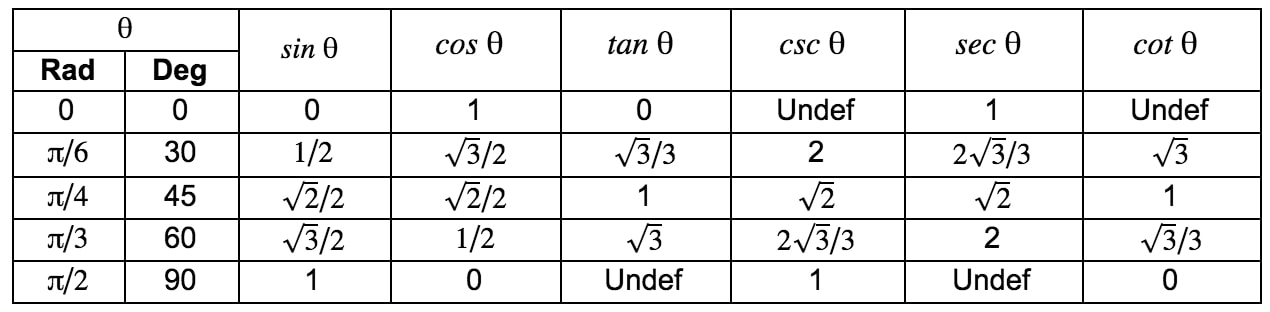
\includegraphics[width=\textwidth]{chart-of-common-trigonometric-ratios-new.jpg}

\end{document}